\documentclass[tikz,border=10pt]{standalone}
\begin{document}

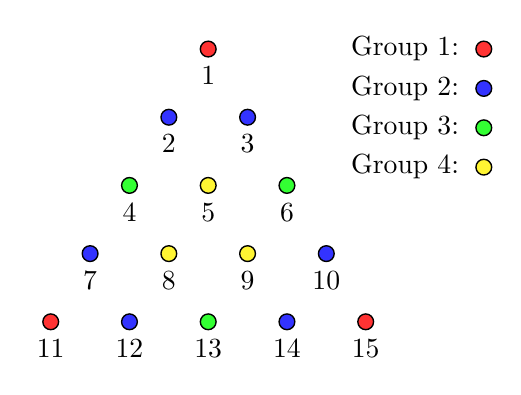
\begin{tikzpicture}

\tikzset{mycircle/.style={fill=red!80!white, draw=black, line width=0.5pt}}
\tikzset{mynode/.style={anchor=north, yshift = -0.1cm, text=black}}

\filldraw[fill=red!80!white, draw=black, line width=0.5pt] (0,0) circle (0.1cm) node[mynode] {$1$};
\filldraw[fill=blue!80!white, draw=black, line width=0.5pt] (-0.5, -0.866) circle (0.1cm) node[mynode] {$2$};
\filldraw[fill=blue!80!white, draw=black, line width=0.5pt] (0.5,-0.866) circle (0.1cm) node[mynode] {$3$};
\filldraw[fill=green!80!white, draw=black, line width=0.5pt] (-1,-1.732) circle (0.1cm) node[mynode] {$4$};
\filldraw[fill=yellow!80!white, draw=black, line width=0.5pt] (0,-1.732) circle (0.1cm) node[mynode] {$5$};
\filldraw[fill=green!80!white, draw=black, line width=0.5pt] (1,-1.732) circle (0.1cm) node[mynode] {$6$};
\filldraw[fill=blue!80!white, draw=black, line width=0.5pt] (-1.5,-2.598) circle (0.1cm) node[mynode] {$7$};
\filldraw[fill=yellow!80!white, draw=black, line width=0.5pt] (-0.5,-2.598) circle (0.1cm) node[mynode] {$8$};
\filldraw[fill=yellow!80!white, draw=black, line width=0.5pt] (0.5,-2.598) circle (0.1cm) node[mynode] {$9$};
\filldraw[fill=blue!80!white, draw=black, line width=0.5pt] (1.5,-2.598) circle (0.1cm) node[mynode] {$10$};
\filldraw[fill=red!80!white, draw=black, line width=0.5pt] (-2,-3.464) circle (0.1cm) node[mynode] {$11$};
\filldraw[fill=blue!80!white, draw=black, line width=0.5pt] (-1,-3.464) circle (0.1cm) node[mynode] {$12$};
\filldraw[fill=green!80!white, draw=black, line width=0.5pt] (0,-3.464) circle (0.1cm) node[mynode] {$13$};
\filldraw[fill=blue!80!white, draw=black, line width=0.5pt] (1,-3.464) circle (0.1cm) node[mynode] {$14$};
\filldraw[fill=red!80!white, draw=black, line width=0.5pt] (2,-3.464) circle (0.1cm) node[mynode] {$15$};



\node at (2.5,0) {Group 1: };
\filldraw[fill=red!80!white, draw=black, line width=0.5pt]
    (3.5,0) circle (0.1cm);

\node at (2.5,-0.5) {Group 2:};
\filldraw[fill=blue!80!white, draw=black, line width=0.5pt]
    (3.5,-0.5) circle (0.1cm);

\node at (2.5,-1) {Group 3:};
\filldraw[fill=green!80!white, draw=black, line width=0.5pt]
    (3.5,-1) circle (0.1cm);

\node at (2.5,-1.5) {Group 4:};
\filldraw[fill=yellow!80!white, draw=black, line width=0.5pt]
    (3.5,-1.5) circle (0.1cm);

\end{tikzpicture}

\end{document}